\documentclass{article}

\usepackage[T1]{fontenc}
\usepackage[utf8]{inputenc}
\usepackage[french,english]{babel}

\usepackage[ruled,lined,commentsnumbered]{algorithm2e}

%% This package is necessary to use \includegraphics.
\usepackage{graphicx}

%% This package is necessary to define hyperlinks.
\usepackage{hyperref}

%% These packages are necessary to include code.
\usepackage{listings}
\usepackage{minted} % colored

%% This package is needed to enchance mathematical formulas.
\usepackage{amsmath}



% This is a comment line in latex

% Latex allows you to define your own "commands",
% better known as "macros" in the Latex world.
% The following line is an example of such definition.
\newcommand{\latex}{\LaTeX}


% The next lines contain some meta informations about this document.

\title{Rapport intermédiaire}
%\subtitle{A minimal demonstration of \latex}

\author{LI Ningyu, WANG Wenchi}


%% Here we begin giving the actual content o the document.
\begin{document}
\maketitle

\selectlanguage{french}

\section{Présentation générale}
Le lancer de rayons (ray tracing) est une technique de simulation de la propagation de la lumière. Il permet notamment d’introduire des ombres portées pour les objets, des réflexions et réfractions entre objets, et des objets transparents. Il consiste à simuler le parcours inverse de la lumière : on calcule les éclairages de la caméra vers les objets puis vers les lumières, alors que dans la réalité la lumière va de la scène vers l'œil.

Dans ce projet, le but est de de programmer un lanceur de rayon lisant un fichier 3D de format OBJ qui contient des objets différents (selon le forme et la texture) et sortant le résultat dans une iamge de 2D. Au premier temps, nous le réaliserons en style "Whitted" avec le modèle "Blinn-Phong", et puis afin de simuler un scénario plus réaliste, nous profiterons de l'illumination globale en base de la théorie radiométrie.

\section{Code implémenté}

Nous utilisons un algorithme principal du lanceur de rayon. Il s’agit de voir le monde avec les yeux plutôt que de voir comment le monde parvient aux yeux. Du côté de la vue, nous envoyons un rayon lumineux vers chaque pixel de l’image, nous traçons ce chemin lumineux et calculons la direction de son rayon inverse, en le mettant sur le pixel correspondant. En calculant la décroissance de la couleur et la superposition sur le trajet de la lumière, la couleur de chaque pixel peut être essentiellement déterminée.

Le traçage de rayons peut être considéré comme un processus récursif. Un rayon est émis dans la scène, l’intersection la plus proche entre le rayon et la géométrie est trouvée, et si le matériau à cette intersection est réfléchissant ou réfringent, le rayon peut être tracé dans la direction de la réflexion ou de la réfraction, et ainsi de suite, de manière récursive, jusqu’à la source de lumière (ou la couleur de fond), et la valeur de coloration de chaque pixel est calculée.

\begin{algorithm}[H]
  \SetAlgoLined
  \KwIn{rayon lumineux}
  \KwOut{couleur du rayon inverse }

  Function tracing():
  
    \eIf{non intersection avec aucun objet}{
      retourner couleur de fond\;
      }{
      obj ← trouver l’objet le plus proche du rayon\;
      rayon réfléchissant ← getRayonReflect(obj)\;
      rayon réfractaire ← getRayonRefract(obj)\;
      couleur principal ← le rayonnement de l'obj\;
      couleur réfléchissant ← tracing(rayon réfléchissant)\;
      couleur réfractaire ← tracing(rayon réfractaire)\;
      }
    
  \caption{Algorithme Récursif Ray Tracer}
\end{algorithm}

Jusqu'à présent, nous avons réalisé le traçage de rayons de plusieurs sphères dans un espace 3D. Chaque sphère peut être réglée sur une taille, un matériau et des coordonnées différents. Nous avons également implémenté l'anti-aliasing de l'image et le déplacement de la position de la caméra.

\begin{figure}[H] 
\centering 
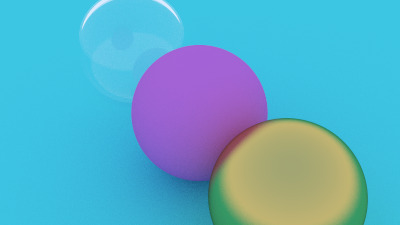
\includegraphics[width=0.7\textwidth]{resultat.jpg} 
\caption{résultat d'exécution} 
\end{figure}



\section{Difficultés rencontrées}

\begin{itemize}
\item L'une des difficultés est de trouver l'objet le plus proche du rayon. Pour cette question, Nous avons créé une classe abstraite "Touché" ayant une fonction "touché" qui prend en compte un rayon. Dans cette classe nous utilisons une structure "touche\_enreg" pour enregistrer les informations d'intersection. Lorsqu'il v1 a plusieurs objets dans la scène, notre approche consiste à itérer à travers tous les objets à chaque intersection. Nous avons besoin d'une "Liste\_touche" pour stocker ces objets. Un rayon émis peut croiser plus d'un objet et nous devons prendre le point d'intersection le plus proche. Cette distance est décrite par "t" dans l'équation du rayon. Évidemment, plus "t" est grand, plus l'intersection est éloignée. Par conséquent, "plusProche" est utilisé pour enregistrer le t minimum de l'intersection actuellement acquise, de sorte que l'intersection la plus proche est nécessairement celle qui est trouvée à la fin.
\item Une autre est de trouver l'intersection entre les rayons et les objets du fichier OBJ. Pour l'instant, nous calculons l'intersection avec le façon suivant : nous présentons un point sur le rayon à une fonction $p(t)=S+tV$, et une sphère à une fonction $(P-c)^{2}=R^{2}$, l'intersection sera la racine du fonction $V^{2}t^{2}+2(V(S-c))t+(S-c)(S-c)-R^{2}=0$. Mais dans le fichier OBJ, il ne stocke que les informations de point, normal et surface. Cette façon ne marche plus, nous n'avons pas encore trouvé une bonne solution pour ce problème. 
\end{itemize}

\section{Prochaines étapes}

\begin{itemize}
\item Essayez d'ajouter d'autres formes d'objets 3D (cubes et rectangles);
\item Mise en œuvre d'une resoursse de lumière;
\item Implémentez un fichier .obj qui stocke toutes les informations 3D de l'objet;
\item À ce stade, pour faciliter la compréhension, nous stockons les informations de la sphère dans le centre et le rayon de la sphère, mais nous devons changer cela pour stocker les informations de la sphère dans les sommets et les normales afin qu'elles puissent être ajoutées au fichier .obj;
\item Mise en œuvre de plusieurs threads pour calculer les valeurs de lumière simultanément.
\end{itemize}


\end{document}
